%
\begin{isabellebody}%
\setisabellecontext{upshot}%
%
\isadelimtheory
%
\endisadelimtheory
%
\isatagtheory
%
\endisatagtheory
{\isafoldtheory}%
%
\isadelimtheory
%
\endisadelimtheory
%
\isadelimdocument
%
\endisadelimdocument
%
\isatagdocument
%
\isamarkupsection{Philosophical Contributions%
}
\isamarkuptrue%
%
\endisatagdocument
{\isafolddocument}%
%
\isadelimdocument
%
\endisadelimdocument
%
\begin{isamarkuptext}%
I argue that computational ethics should be useful for and interesting to philosophers for two 
reasons. First, it serves as the basis for AI agents with the capacity for philosophically sophisticated 
ethical reasoning. For example, my project contributes an implementation of the Formula of Universal Law
that an AI agent could use to reason about the world using the categorical imperative. Second, computational 
ethics helps philosophers think about ethics in the same way that calculators or theorem provers help 
mathematicians think about math. I am not arguing that the computer can replace human reasoning or prove things
that humans theoretically couldn't do. Instead, I argue that the computer bolsters human reasoning, firstly by forcing precision due to 
the rigid syntax of a computer program and secondly by making formal proofs less tedious. Below, I explore each of 
these contributions in greater detail.%
\end{isamarkuptext}\isamarkuptrue%
%
\isadelimdocument
%
\endisadelimdocument
%
\isatagdocument
%
\isamarkupsubsection{AI Agents%
}
\isamarkuptrue%
%
\endisatagdocument
{\isafolddocument}%
%
\isadelimdocument
%
\endisadelimdocument
%
\begin{isamarkuptext}%
As artifical intelligence becomes more powerful, science fiction looms closer to reality and the 
danger of ``unethical" AI becomes more urgent. Ethically intelligent artificial agents will need to 
be able to reason about sophisticated ethical theories in order to navigate the world. My project could 
serve as one component of a complete ethical reasoner. Specifically, my project could easily be repurposed 
into a library or ``engine" that takes as input the logical representation of a maxim and determines if it is obligatory, prohibited, 
or permissible.

As it stands, my project can evaluate the moral status of maxims represented in my logic and potentially 
serves as one component of an ``ethics engine," which an AI agent could use to make ethical decisions.
For example, my system could be combined with an input parser to translate moral dilemmas or situations into maxims in my logic and an output 
to translate the moral status output of my system into a prescription for what action should be taken.
The diagram below depicts the workflow of this example of an ethics engine.%
\end{isamarkuptext}\isamarkuptrue%
%
\begin{figure}
\centering
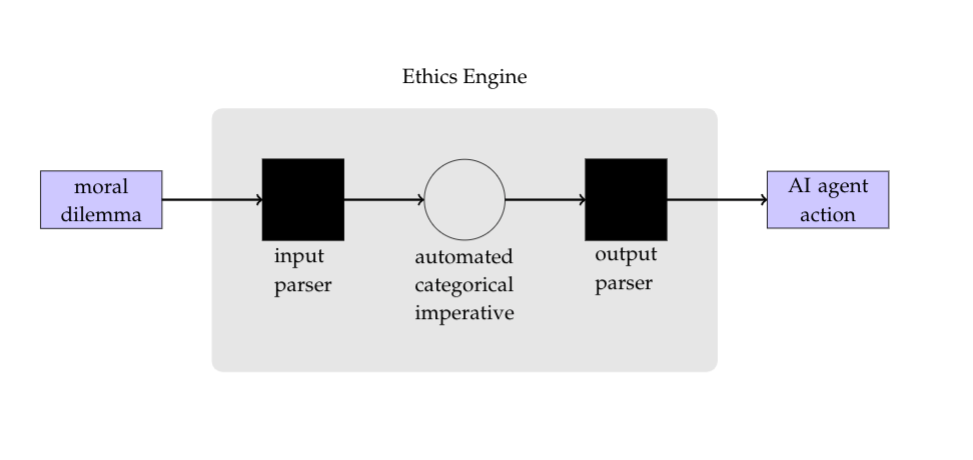
\includegraphics[scale=0.4]{AI_engine.png}
\caption{An example of an ethics engine for an artificial agent} \label{fig:1}
\end{figure}
%
\begin{isamarkuptext}%
In this workflow, an AI agent is faced with a moral dilemma in some internal representation and 
passes this representation to a parser, which converts it to the appropriate logical representation 
for my system to evaluate. For example, if an AI agent represents the moral dilemma in natural language, 
the parser would convert the natural language representation to a representation in my logic.

Once the
input is a sentence in my logic, my project can evaluate its moral status using my implementation of 
the FUL. Concretely, my project would return a value indicating if the maxim is obligatory, permissible, 
or prohibited. The maxim would be prohibited if it fails the universalizability test, permissible if it passes, and obligatory 
if its negation fails the universalizability test. All three of these properties amount to testing if a 
certain theorem holds or not in my logic, a calculation that I demonstrate repeatedly in my tests. 

This output could then be converted into some actionable, useful response for the AI agent with another 
output parser. For example, if the AI agent is equipped to evaluate natural language prescriptions, the 
status of the maxim could be parsed into a natural language sentence. This output will be passed back 
to the AI agent, which will make a decision using it.

The ethics engine depicted above is merely one way to use my project to guide an artifical agent. The 
upshot is that an automated version of the categorical imperative could function as the ethical engine 
for an AI agent, with some work to parse the input and the output. Effectively, some version of the kind 
of automated ethics I implement could be 
exposed as an ``ethics API" that AI developers could use to easily give AI agent the capacity for 
sophisticated ethical reasoning faithful to philosophical literature. This represents an improvement 
over existing ethics engines, which, as I examine in Section ??, rarely attempt to capture the complexity 
of any ethical theory that philosophers plausibly defend.%
\end{isamarkuptext}\isamarkuptrue%
%
\isadelimdocument
%
\endisadelimdocument
%
\isatagdocument
%
\isamarkupsubsection{Computational Philosophy%
}
\isamarkuptrue%
%
\isamarkupsubsubsection{Example of a  Philosophical Insight%
}
\isamarkuptrue%
%
\endisatagdocument
{\isafolddocument}%
%
\isadelimdocument
%
\endisadelimdocument
%
\begin{isamarkuptext}%
As I tested prior formulations of the categorical imperative and implemented my own, the process 
of implementing a formalization and testing it using an interactive theorem prover resulted in philosophical 
insights that were novel to me. The process resulted in surprising logical results that provoked 
interesting philosophical conversations as I tried to understand their implications for the ethical 
theory I am formalizing. 

For example, as I was implementing my formalization of the FUL, I realized
that my formalization was inconsistent unless I specified that the FUL only held for ``well-formed maxims,"
such that neither the act nor goal were already achieved in the given circumstances. Below I document how 
I came to this conclusion. First, I used Sledgehammer to show that my formalization of the FUL\footnote{The full logical representation is \isa{FUL{\isadigit{0}}\ {\isasymequiv}\ {\isasymforall}c\ a\ g\ s{\isachardot}\ not{\isacharunderscore}universalizable\ {\isacharparenleft}c{\isacharcomma}\ a{\isacharcomma}\ g{\isacharparenright}\ s\ {\isasymlongrightarrow}\ {\isasymTurnstile}prohibited\ {\isacharparenleft}c{\isacharcomma}\ a{\isacharcomma}\ g{\isacharparenright}\ s}.}
resulted in a contradiction. Sledgehammer was able to tell me which axioms it used to complete 
this proof, showing me that my formalization contradicted the axiom O\_diamond, which states that an 
obligated term cannot contradict its context. I hypothesized that there was some tension between 
the antecedent of the FUL, which states that a maxim is acted on by all agents, and the consequent, 
which states that a maxim is prohibited. If the maxim has already been acted on, then not acting on it
becomes impossible so the prohibition is impossible to obey! 

To solve this problem, I returned to Korsgaard's practical contradiction interpretation and focused 
on the imaginatory component of the FUL. Specifically, the universalizability test requires that we IMAGINE 
a world where the maxim is universalized, not that the maxim is actually universalized at this world. 
I implemented another version of the FUL under which, if a maxim is universalized at any world and rendered
ineffective at that world, it is prohibited at the current world. I hypothesized that this would remove 
the contradiction found above. However, Nitpick was still timing out when looking for a model that
satisfied this new version of the FUL. Nitpick is a model checker that generates models that satisfy 
some axioms and theorems, and usually it is able to find small satisfying models in a matter of seconds. 
The fact that Nitpick was timing out was a serious indication that my formalization was still not 
consistent.

I suspected that Nitpick could possibly be timing out due to checking large models that exhausted its 
time limit. To avoid this, I decided to help the system out and specify the exact number of maxims 
in the system by passing as an argument to Nitpick the cardinality of my desired model. This did not 
fix the problem. I next defined a particular (circumstance, act, goal) tuple as a constant and, instead of
stating that the FUL held for all maxims, I stated that the FUL held for the specific maxim formed by this tuple.
To my surprise, Nitpick was now able to show that the FUL was consistent!

This initially appeared counterintuitive—after all, what is the difference between a model of cardinality 
1 and a model with one constant object? Professor Amin pointed out that as constants, the circumstances, 
act, and goal for which the FUL held were all distinct, but when quantified over they were not. One line 
of code later, I tested this hypothesis and found that, indeed, specifying that the circumstances could 
not entail the act or goal fixed the inconsistency! This logical inconsistency showed me that the FUL 
could not hold for maxims in which the act or goal have already been achieved in the circumstances.

To understand this property as a philoosphical insight, I returned to Korsgaard and O'Neill's 
interpretations of maxims as practical, action-guiding principles, and concluding that a maxim in 
which the circumstances already entail the act or goal is vacuous and not a useful practical principle 
to evaluate. This is a non-trivial philosophical insight that the computer helped me discover!%
\end{isamarkuptext}\isamarkuptrue%
%
\isadelimdocument
%
\endisadelimdocument
%
\isatagdocument
%
\isamarkupsubsubsection{Two Uses of Computational Ethics%
}
\isamarkuptrue%
%
\endisatagdocument
{\isafolddocument}%
%
\isadelimdocument
%
\endisadelimdocument
%
\begin{isamarkuptext}%
I do not argue that computational ethics uncovers philosophical insights that humans have not reached 
or are incapable of reaching. After all, my understanding of a well-formed maxim could 
very well exist in the literature and certainly could be reached by a philosopher working without any 
computational tools. Instead, I argue that computational tools prompt philosophers to ask questions that 
lead to insights. The computer offers a different perspective by forcing philosophers to make their 
work precise and allowing them to quickly complete proofs that would otherwise be tedious.

Representing a philosophical idea in logic and implementing it in an interactive theorem prover requires 
making the idea precise to a degree that ordinary discussion does not require. The initial representation 
of an idea in a logic requires extracting the essence of the idea and making its form precise. For example, 
as I formalized the notion of a maxim, I had to understand its components and make its form as a 
circumstance, act, goal tuple precise. Moreover, Isabelle's strict typing system required that I define 
coherent, consistent types for each of these entities and for a maxim as a whole. This requires understanding 
what role each of these components play in the FUL and assigning them each a type. In my example, I 
concluded that circumstances and goals are terms, which can be true or false at a world, and acts are 
open sentences, which are true for a particular subject at a particular world. This precision is possible 
without computational tools, but computational ethics forces a level of precision that ordinary discussion 
does not demand. Type fuzziness and overloaded definitions are all too common in philosophical writing and 
discussion (would be cool to cite some famous debate revolving around this idea), but computers don't 
allow this kind of imprecision.

The second virtue of computational ethics is that it makes formal ethics far less tedious, and therefore 
within reach even for non-logicians. There is plenty of work attempting to develop logical representations 
of philosophical phenomena in order to make these phenomena precise and use the tools of logic to prove 
facts about them. Much of this work, however, requires tedious pencil and paper proofs which may not 
always produce relevant philosophical insights. Interactive theorem provers make such proofs accessible 
even to philosophers who don't specialize in logic. Moreover, these proofs start from first principles 
without requiring that a human being write pages and pages of syllogism as in Principia Mathematica. 
Just as calculators make arithmetic fast and accessible to non-specialists, computational ethics does the same for 
formal philosophy.%
\end{isamarkuptext}\isamarkuptrue%
%
\isadelimdocument
%
\endisadelimdocument
%
\isatagdocument
%
\isamarkupsubsubsection{Looking Forward%
}
\isamarkuptrue%
%
\endisatagdocument
{\isafolddocument}%
%
\isadelimdocument
%
\endisadelimdocument
%
\begin{isamarkuptext}%
My project does not demonstrate that computational ethics can discover new philosophical 
insights that humans are incapable of reaching. After all, my understanding of a well-formed maxim could 
very well exist in the literature and certainly could be reached by a philosopher working without any 
computational tools. Instead, the upshot is that working with a computer, today, is another way for 
philosophers to arrive at philosophical insights. Just as theorem provers do not replace mathematicians 
entirely, computational ethics does not outdo the philosopher but instead helps them do their work faster. 
The computer offers a different perspective and prompts new questions that lead to insights. 


Computational ethics is at its infancy. The use of theorem provers in mathematics is just now beginning 
to make headway (cite Kevin Buzzard), even though theorem provers were first invented in the 1960's (cite 
https://www.cl.cam.ac.uk/~jrh13/papers/joerg.pdf). In contrast, the first attempts to use theorem 
provers for ethics occurred in the last decade. The fact that this nascent technology is already 
helping humans reach non-trivial philosophical conclusions is reason to, at the very least, entertain 
the possibility of a future where computational ethics becomes as normal as using a calculator for arithmetic.

To the skeptic, the ethical insights uncovered by the computer are not necessarily trendy or impressive 
philosophy. Indeed, the fact that a theorem prover requires specialized knowledge outside of the field 
of philosopher indicates that the technology is nowhere near ready for universal use in philosophy 
departments. However, history indicates that as computing power increases and computer scientists make 
progress, computational ethics will become more usable. Theorem provers in mathematics began as toys 
incapable of proving that the real number 2 is not equal to the real number 1, but Buzzard showed that 
moving from such a primitive system to a tool for Fields medal winning mathematics is possible in a 
matter of years (cite Buzzard). Countless examples from the history of computer science, from the Turing 
Test to AI game playing to protein folding, demonstrate that progress in computer science can make seemingly 
obscure computer programs useful and usable in ways that exceed our wildest imaginations. Indeed, 
programmable computers themselves initially began as unwieldy punch card readers, but their current ubiquity 
need not be stated. If computer scientists and philosophers invest in computational ethics, it can 
become as much a tool for philosophy as a calculator is for for arithmetic.\footnote{Is this too like, 
lalalala fantasy of computational philosophy?}%
\end{isamarkuptext}\isamarkuptrue%
%
\isadelimtheory
%
\endisadelimtheory
%
\isatagtheory
%
\endisatagtheory
{\isafoldtheory}%
%
\isadelimtheory
%
\endisadelimtheory
%
\end{isabellebody}%
\endinput
%:%file=~/Desktop/cs91r/paper/upshot.thy%:%
%:%24=6%:%
%:%36=8%:%
%:%37=9%:%
%:%38=10%:%
%:%39=11%:%
%:%40=12%:%
%:%41=13%:%
%:%42=14%:%
%:%43=15%:%
%:%44=16%:%
%:%53=18%:%
%:%65=20%:%
%:%66=21%:%
%:%67=22%:%
%:%68=23%:%
%:%69=24%:%
%:%70=25%:%
%:%71=26%:%
%:%72=27%:%
%:%73=28%:%
%:%74=29%:%
%:%75=30%:%
%:%76=31%:%
%:%79=35%:%
%:%80=36%:%
%:%81=37%:%
%:%82=38%:%
%:%83=39%:%
%:%86=41%:%
%:%87=42%:%
%:%88=43%:%
%:%89=44%:%
%:%90=45%:%
%:%91=46%:%
%:%92=47%:%
%:%93=48%:%
%:%94=49%:%
%:%95=50%:%
%:%96=51%:%
%:%97=52%:%
%:%98=53%:%
%:%99=54%:%
%:%100=55%:%
%:%101=56%:%
%:%102=57%:%
%:%103=58%:%
%:%104=59%:%
%:%105=60%:%
%:%106=61%:%
%:%107=62%:%
%:%108=63%:%
%:%109=64%:%
%:%110=65%:%
%:%119=67%:%
%:%123=69%:%
%:%135=71%:%
%:%136=72%:%
%:%137=73%:%
%:%138=74%:%
%:%139=75%:%
%:%140=76%:%
%:%141=77%:%
%:%142=78%:%
%:%143=79%:%
%:%144=80%:%
%:%145=81%:%
%:%146=82%:%
%:%147=83%:%
%:%148=84%:%
%:%149=85%:%
%:%150=86%:%
%:%151=87%:%
%:%152=88%:%
%:%153=89%:%
%:%154=90%:%
%:%155=91%:%
%:%156=92%:%
%:%157=93%:%
%:%158=94%:%
%:%159=95%:%
%:%160=96%:%
%:%161=97%:%
%:%162=98%:%
%:%163=99%:%
%:%164=100%:%
%:%165=101%:%
%:%166=102%:%
%:%167=103%:%
%:%168=104%:%
%:%169=105%:%
%:%170=106%:%
%:%171=107%:%
%:%172=108%:%
%:%173=109%:%
%:%174=110%:%
%:%175=111%:%
%:%176=112%:%
%:%177=113%:%
%:%178=114%:%
%:%179=115%:%
%:%180=116%:%
%:%189=118%:%
%:%201=120%:%
%:%202=121%:%
%:%203=122%:%
%:%204=123%:%
%:%205=124%:%
%:%206=125%:%
%:%207=126%:%
%:%208=127%:%
%:%209=128%:%
%:%210=129%:%
%:%211=130%:%
%:%212=131%:%
%:%213=132%:%
%:%214=133%:%
%:%215=134%:%
%:%216=135%:%
%:%217=136%:%
%:%218=137%:%
%:%219=138%:%
%:%220=139%:%
%:%221=140%:%
%:%222=141%:%
%:%223=142%:%
%:%224=143%:%
%:%225=144%:%
%:%226=145%:%
%:%227=146%:%
%:%228=147%:%
%:%229=148%:%
%:%230=149%:%
%:%239=151%:%
%:%251=153%:%
%:%252=154%:%
%:%253=155%:%
%:%254=156%:%
%:%255=157%:%
%:%256=158%:%
%:%257=159%:%
%:%258=160%:%
%:%259=161%:%
%:%260=162%:%
%:%261=163%:%
%:%262=164%:%
%:%263=165%:%
%:%264=166%:%
%:%265=167%:%
%:%266=168%:%
%:%267=169%:%
%:%268=170%:%
%:%269=171%:%
%:%270=172%:%
%:%271=173%:%
%:%272=174%:%
%:%273=175%:%
%:%274=176%:%
%:%275=177%:%
%:%276=178%:%
%:%277=179%:%
%:%278=180%:%
%:%279=181%:%
%:%280=182%:%